\documentclass[10,a4paperpaper,]{article}

  \title{End of Session CKLA Report}
  \author{Teaching Lab}
  \date{\today}
  


\newcommand{\logo}{teachinglab_logo.png}
\newcommand{\cover}{cover.png}
\newcommand{\iblue}{04abeb}
\newcommand{\igray}{d4dbde}
\usepackage{amsmath}
\usepackage{booktabs}
\usepackage{caption}
\usepackage{longtable}

% Author: Karol KozioL
% License: GPL-3
% Modified by: Sarah Wagner

% % % packages -----------------------------------------------------------------------------------
\usepackage{amsmath}
\usepackage{array}
\usepackage{booktabs}
\usepackage{calc}
\usepackage{eso-pic}
\usepackage{fancyhdr}
\usepackage{fontspec}
\usepackage[left = 2.5cm, right = 2.5cm, top = 1.2cm, bottom = 1.2cm, includeheadfoot]{geometry}
\usepackage{graphicx}
\usepackage[utf8]{inputenc}
\usepackage{lastpage}
\usepackage{multirow}
\usepackage{tabularx} 
\usepackage{tikz}
\usepackage{titlesec}
\usepackage{xcolor, colortbl}

% % % settings -----------------------------------------------------------------------------------

% % custom colors
\definecolor{iblue}{HTML}{\iblue}
\definecolor{igray}{HTML}{\igray}
% % empty tightlist fix
\def\tightlist{}

% definition of pagename
\newcommand\pagename{Page}

% % fonts 
\defaultfontfeatures{Mapping = tex-text}
\setmainfont[BoldFont = calibri-bold.otf, ItalicFont = calibri-italic.otf, BoldItalicFont = calibri-bold-italic.otf]{calibri.otf}
\newfontfamily\headingfont[ItalicFont = calibri-italic.otf]{calibri.otf}


% % sections
\titleformat{\section}{\color{iblue}\headingfont\Large\bfseries}{\thesection}{1em}{}[\titlerule]
\titleformat{\subsection}{\color{iblue}\headingfont\large\bfseries}{\thesubsection}{1em}{}
\titleformat{\subsubsection}{\color{iblue}\headingfont\bfseries}{\thesubsubsection}{1em}{}

% % misc
\setlength{\parindent}{0em} 
\linespread{1}
\raggedright
\newcolumntype{C}{>{\centering\arraybackslash}X}


% % % custom titlepage ----------------------------------------------------------------------------
\newcommand\BackgroundPic{%
	\put(0,0){%
		\parbox[b][\paperheight]{\paperwidth}{%
			\vfill
			\centering
			
\includegraphics[width=\paperwidth,height=\paperheight]{\cover}%
			\vfill
}}}

\makeatletter

% pagestyle titlepage
\fancypagestyle{customtitle}{
	\lhead{}
	\chead{}
	\rhead{}
	\makeatother
	\lfoot{}
	\cfoot{}
	\rfoot{
\includegraphics{\logo}}
}


% titlepage
\renewcommand{\maketitle}{
	\thispagestyle{customtitle}
	\AddToShipoutPicture*{\BackgroundPic}
	\ClearShipoutPicture
	
	\phantom{a}\hfill
	\vspace{14cm}
	
	\begin{tabular}[l]{@{}p{\textwidth}@{}}
		\color{iblue}\headingfont\LARGE\@title\\[1em]
		\color{iblue}\headingfont\large\@author\\[1em]
		\color{iblue}\headingfont\small\@date\\[1em]
	\end{tabular}
	
	
	
	\clearpage
}
\makeatother

% % % header and footer ---------------------------------------------------------------------------
\pagestyle{fancy}
\lhead{}
\chead{}
\rhead{ 
\includegraphics{\logo}}
\makeatother
\newlength{\myheight}
\lfoot{}
\cfoot{}
\rfoot{\pagename~\thepage \hspace{1pt} / \pageref{LastPage}}
\renewcommand\headrulewidth{0pt}
\renewcommand\footrulewidth{0pt}




\begin{document}


\renewcommand{\contentsname}{Table of Contents}

\renewcommand{\pagename}{Page}


\maketitle
\tableofcontents
\addcontentsline{toc}{section}{Contents}

\section{Facilitation Reviews}

\begin{center}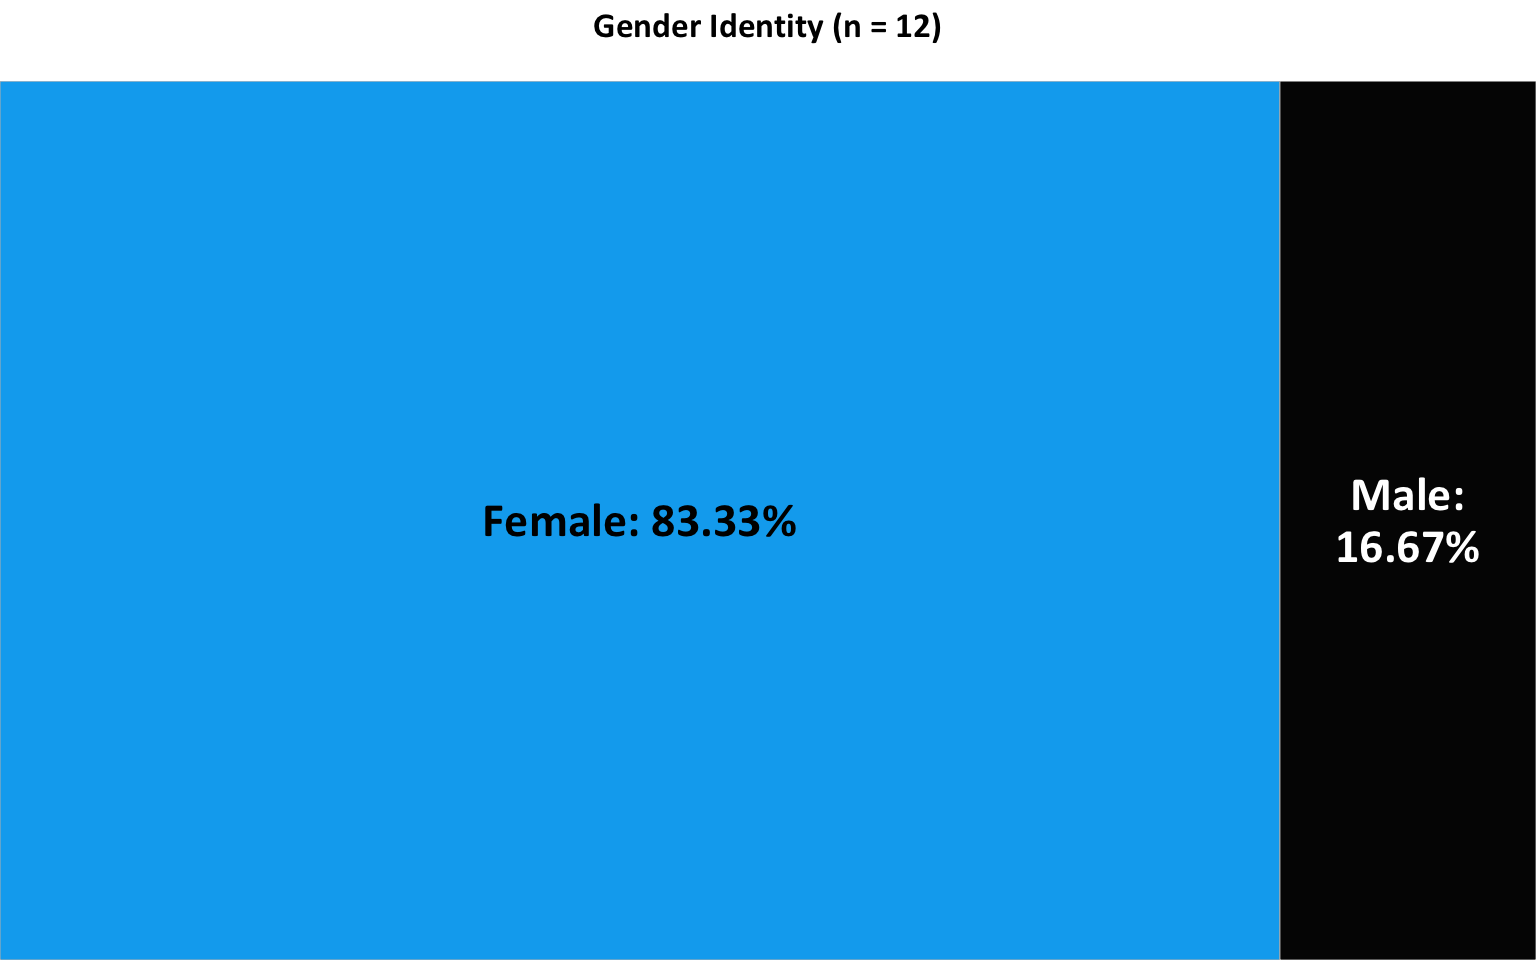
\includegraphics{/Users/dunk/Teaching Lab/Coding/TeachingLab/Analysis/2022-2023/Reports/reports_generated/provide_data_pdf_report_session_files/figure-latex/unnamed-chunk-1-1} \end{center}

\subsection{Percent Agree and Strongly Agree}

In summary, we see the following \% agree or strongly agree with the
above statements:

\begin{itemize}
\tightlist
\item
  \% strongly agree or agree that the facilitators were fully prepared
  for the session.
\item
  \% strongly agree or agree that the facilitators responded to the
  group's needs.
\item
  \% strongly agree or agree that the facilitators facilitated the
  content clearly.
\item
  \% strongly agree or agree that the facilitators effectively built a
  safe learning community.
\item
  \% strongly agree or agree that the facilitators demonstrated deep
  knowledge of the content they facilitated.
\end{itemize}

\section{Qualitative End of Session Participant Feedback}

Finally responses to the following questions are presented below:

\begin{itemize}
\item
  What is one thing from today's learning that you plan to take back to
  your classroom?
\item
  What went well in today's session?
\item
  What could have been better about today's session?
\item
  Any additional feedback
\end{itemize}

\subsection{What is one thing from today's learning that you plan to take back to your classroom?}

\captionsetup[table]{labelformat=empty,skip=1pt}
\begin{longtable}{c}
\toprule
What is one thing from today's learning that you plan to take back to your classroom? \\ 
\midrule
How to built students\textquotesingle{} background knowledge when introducing a new lesson. \\ 
\bottomrule
\end{longtable}

\subsection{What went well in today's session?}

\captionsetup[table]{labelformat=empty,skip=1pt}
\begin{longtable}{c}
\toprule
What went well in today’s session? \\ 
\midrule
The discussions with had as a group. \\ 
\bottomrule
\end{longtable}

\subsection{What is the learning from this course that you are most excited about trying out?}

\captionsetup[table]{labelformat=empty,skip=1pt}
\begin{longtable}{c}
\toprule
What could have been better about today’s session? \\ 
\midrule
\bottomrule
\end{longtable}

\subsection{Any additional feedback}

\begin{center}
\includegraphics{/Users/dunk/Teaching Lab/Coding/TeachingLab/Analysis/2022-2023/Reports/reports_generated/provide_data_pdf_report_session_files/figure-latex/unnamed-chunk-8-1} \end{center}


\end{document}
